
\begin{frame}{\citetitle{MarcoNuno_ReporteTecnico2022_B}$^*$  (1)}

\begin{columns}
\begin{column}{0.70\textwidth}
	\begin{itemize}
		\item El chile piquín (\textit{Capsicum annuum L. var. aviculare}) es una producto endémico de la región noreste de la república mexicana
        \item Durante la cosecha, el fruto tiene que ser cortado junto con su pedúnculo
        \item Se desarrolló de una máquina que permita quitar el cabo en forma automática para agregar valor a su producción
	\end{itemize}
\end{column}
\begin{column}{0.30\textwidth}  
\begin{center}
     \begin{tabular}{cc}
         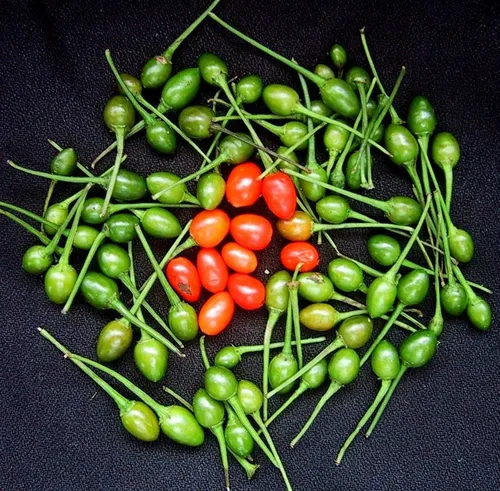
\includegraphics[width=0.68\textwidth]{2022_MaquinaChilePiquin/figs/TeSientas.png}\\         
      \end{tabular}
\end{center}
\end{column} 
\end{columns} 


%\footnotetext[1]{\fullcite{MarcoNuno_ReporteTecnico2022_C}}
%\setcounter{footnote}{0}
\footfullcite*{MarcoNuno_ReporteTecnico2022_B}
\end{frame}


\begin{frame}{\citetitle{MarcoNuno_ReporteTecnico2022_B} (2)}
\begin{columns}
\begin{column}{0.50\textwidth}
Prototipo 1:
\begin{itemize}
        \item Un pistón neumático se accionaba para darle movimiento 
        \item El corte de los pedúnculo era efectuado por unas peinetas estratégicamente colocadas
        \item Llevaba a cabo el corte de manera eficaz, pero requeria del acomodo de los chiles
	\end{itemize}
\end{column}
\begin{column}{0.50\textwidth}  
\begin{center}
     \begin{tabular}{c}
         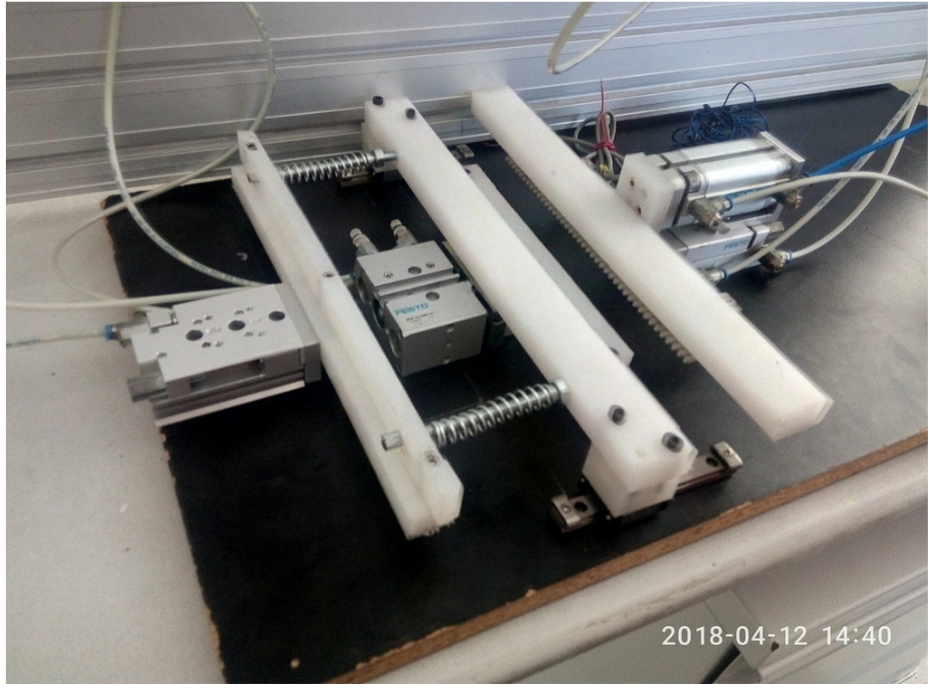
\includegraphics[width=0.98\textwidth]{2022_MaquinaChilePiquin/figs/Prototipo1.png}\\
          \end{tabular}
\end{center}
\end{column} 
\end{columns} 
\end{frame}



\begin{frame}{\citetitle{MarcoNuno_ReporteTecnico2022_B} (3)}
\begin{columns}
\begin{column}{0.55\textwidth}
Prototipo 2:
\begin{itemize}
        \item Se agregaron modificaciones para permitir el posicionamiento de
los chiles sin necesidad de intervención humana. 
        \item Usa sistemas neumáticos y eléctricos para accionar los diferentes mecanismos.
        \item Este prototipo realiza el desprendimiento de los pedúnculos, sin embargo todavía es necesaria la intervención humana para lograr una adecuada remoción de los mismos
	\end{itemize}
\end{column}
\begin{column}{0.45\textwidth}  
\begin{center}
     \begin{tabular}{c}
         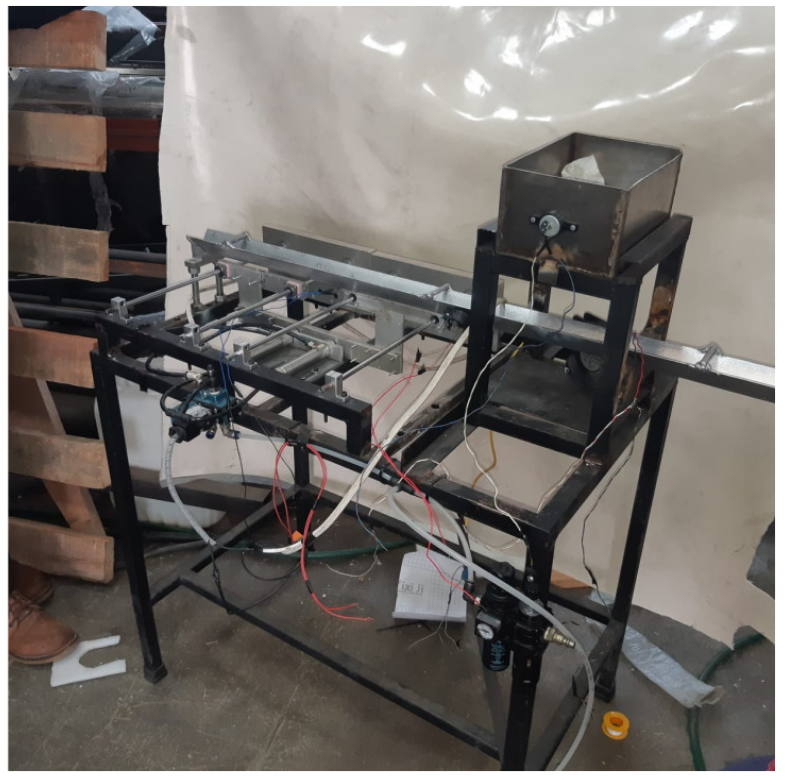
\includegraphics[width=0.98\textwidth]{2022_MaquinaChilePiquin/figs/Prototipo2.png}\\
          \end{tabular}
\end{center}
\end{column} 
\end{columns} 
\end{frame}


\begin{frame}{\citetitle{MarcoNuno_ReporteTecnico2022_B} (4)}
\begin{columns}
\begin{column}{0.60\textwidth}
Prototipo 3:
\begin{itemize}
    \item Un diseño nuevo consiste de una máquina con 3 sistemas: sistema de suministro, sistema de separación y sistema de corte    
    \item Se eliminaron los sistemas neumáticos, usando un solo motor de corriente alterna, además de usar mecanismos fáciles de replicar
    \item Utiliza solo materiales de grado alimenticio como lo son el acero inoxidable y el Nylamid, en la versión industrial
    \item Este prototipo puede desprender los pedúnculos sin importar la posición en la que se recibieran los frutos
	\end{itemize}
\end{column}
\begin{column}{0.40\textwidth}  
\begin{center}
     \begin{tabular}{c}
         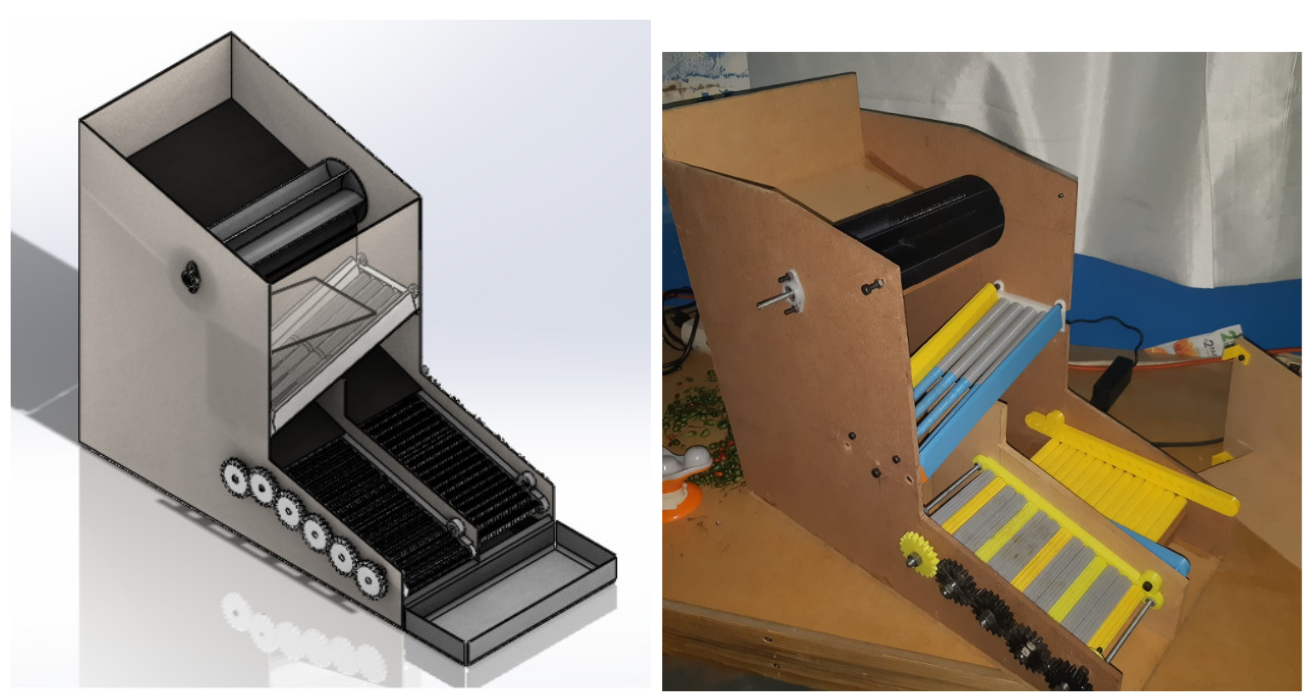
\includegraphics[width=0.98\textwidth]{2022_MaquinaChilePiquin/figs/Prototipo3.png}\\
          \end{tabular}
\end{center}
\end{column} 
\end{columns} 
\end{frame}


\begin{frame}{\citetitle{MarcoNuno_ReporteTecnico2022_B} (5)}
\begin{columns}
\begin{column}{0.70\textwidth}
Prototipo Final:
\begin{itemize}
    \item Actualmente esta en desarrollo, e incluirá los sistemas que funcionaron de los prototipos anteriores
    \item Se incluirá un sensor óptico para medir el rendimiento (cantidad de chiles procesadoss por minuto)
	\end{itemize}
\end{column}
\begin{column}{0.30\textwidth}  
\begin{center}
     \begin{tabular}{c}
         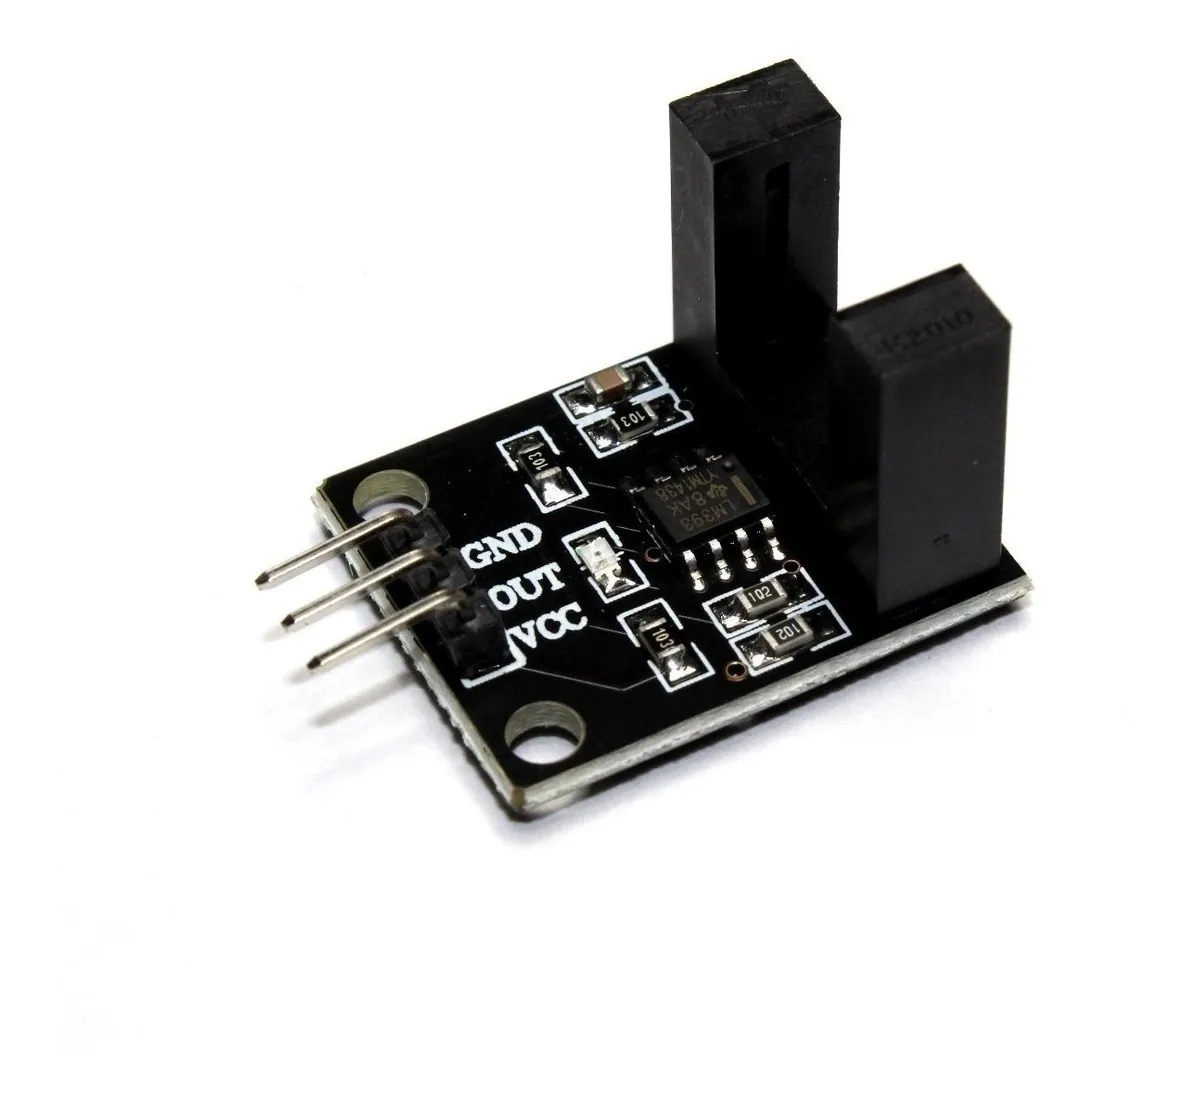
\includegraphics[width=0.98\textwidth]{2022_MaquinaChilePiquin/figs/SensorOptico.png}\\
          \end{tabular}
\end{center}
\end{column} 
\end{columns} 
\end{frame}


